% !TeX program = lualatex
\documentclass[tikz,border=6pt]{standalone}

\usepackage{pgfplots}
\pgfplotsset{compat=1.18}

\begin{document}
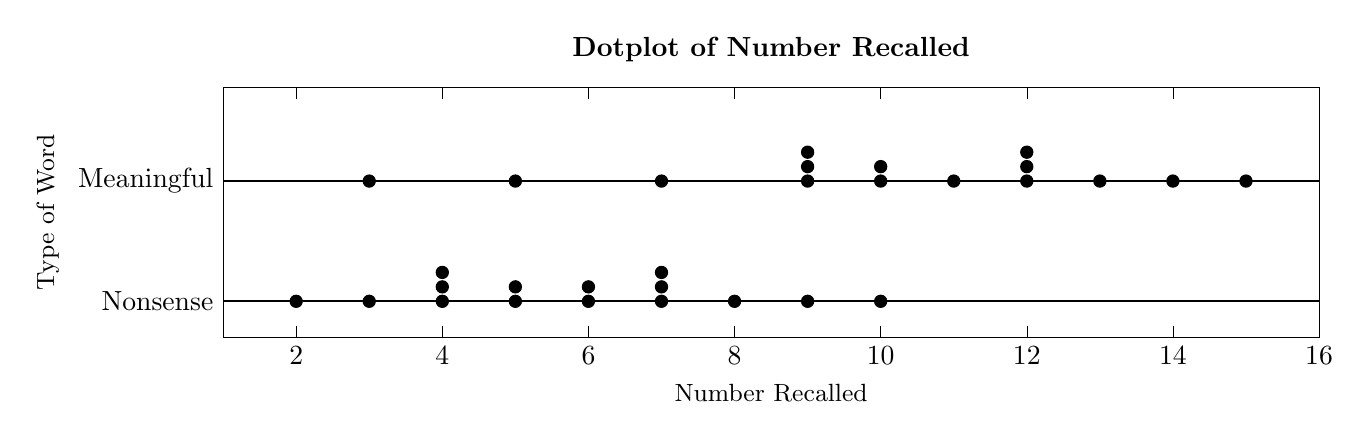
\begin{tikzpicture}

\begin{axis}[
  title={Dotplot of Number Recalled},
  xlabel={Number Recalled},
  ylabel={Type of Word},
  axis lines=box,
  xmin=1, xmax=16,
  ymin=0.7, ymax=2.775,
  xtick={2,4,6,8,10,12,14,16},
  ytick={1,2},
  yticklabels={Nonsense, Meaningful},
  width=15.5cm,
  height=4.75cm,
  tick style={black},
  major tick length=4pt,
  title style={font=\bfseries},
  label style={font=\small}
]

% Hai đường ngang (giống mẫu)
\addplot[black, thick] coordinates {(1,1) (16,1)};
\addplot[black, thick] coordinates {(1,2) (16,2)};

% ------------------------------------------------------------
% Nonsense (baseline y=1), step=0.12
% Data: 4,6,6,5,7,5,4,7,9,10,4,8,7,3,2
% Counts: 2(1),3(1),4(3),5(2),6(2),7(3),8(1),9(1),10(1)
% ------------------------------------------------------------
\addplot[
  only marks,
  mark=*,
  mark size=2.2pt
] coordinates {
  (2,1.00)
  (3,1.00)
  (4,1.00) (4,1.12) (4,1.24)
  (5,1.00) (5,1.12)
  (6,1.00) (6,1.12)
  (7,1.00) (7,1.12) (7,1.24)
  (8,1.00)
  (9,1.00)
  (10,1.00)
};

% ------------------------------------------------------------
% Meaningful (baseline y=2), step=0.12
% Data: 12,15,12,12,10,3,7,11,9,14,9,10,9,5,13
% Counts: 3(1),5(1),7(1),9(3),10(2),11(1),12(3),13(1),14(1),15(1)
% ------------------------------------------------------------
\addplot[
  only marks,
  mark=*,
  mark size=2.2pt
] coordinates {
  (3,2.00)
  (5,2.00)
  (7,2.00)
  (9,2.00) (9,2.12) (9,2.24)
  (10,2.00) (10,2.12)
  (11,2.00)
  (12,2.00) (12,2.12) (12,2.24)
  (13,2.00)
  (14,2.00)
  (15,2.00)
};

\end{axis}
\end{tikzpicture}
\end{document}
